\section{Related Work}

\begin{frame}{Related Work}
       \tableofcontents[sectionstyle=show/hide, hideothersubsections]
    \begin{center}
    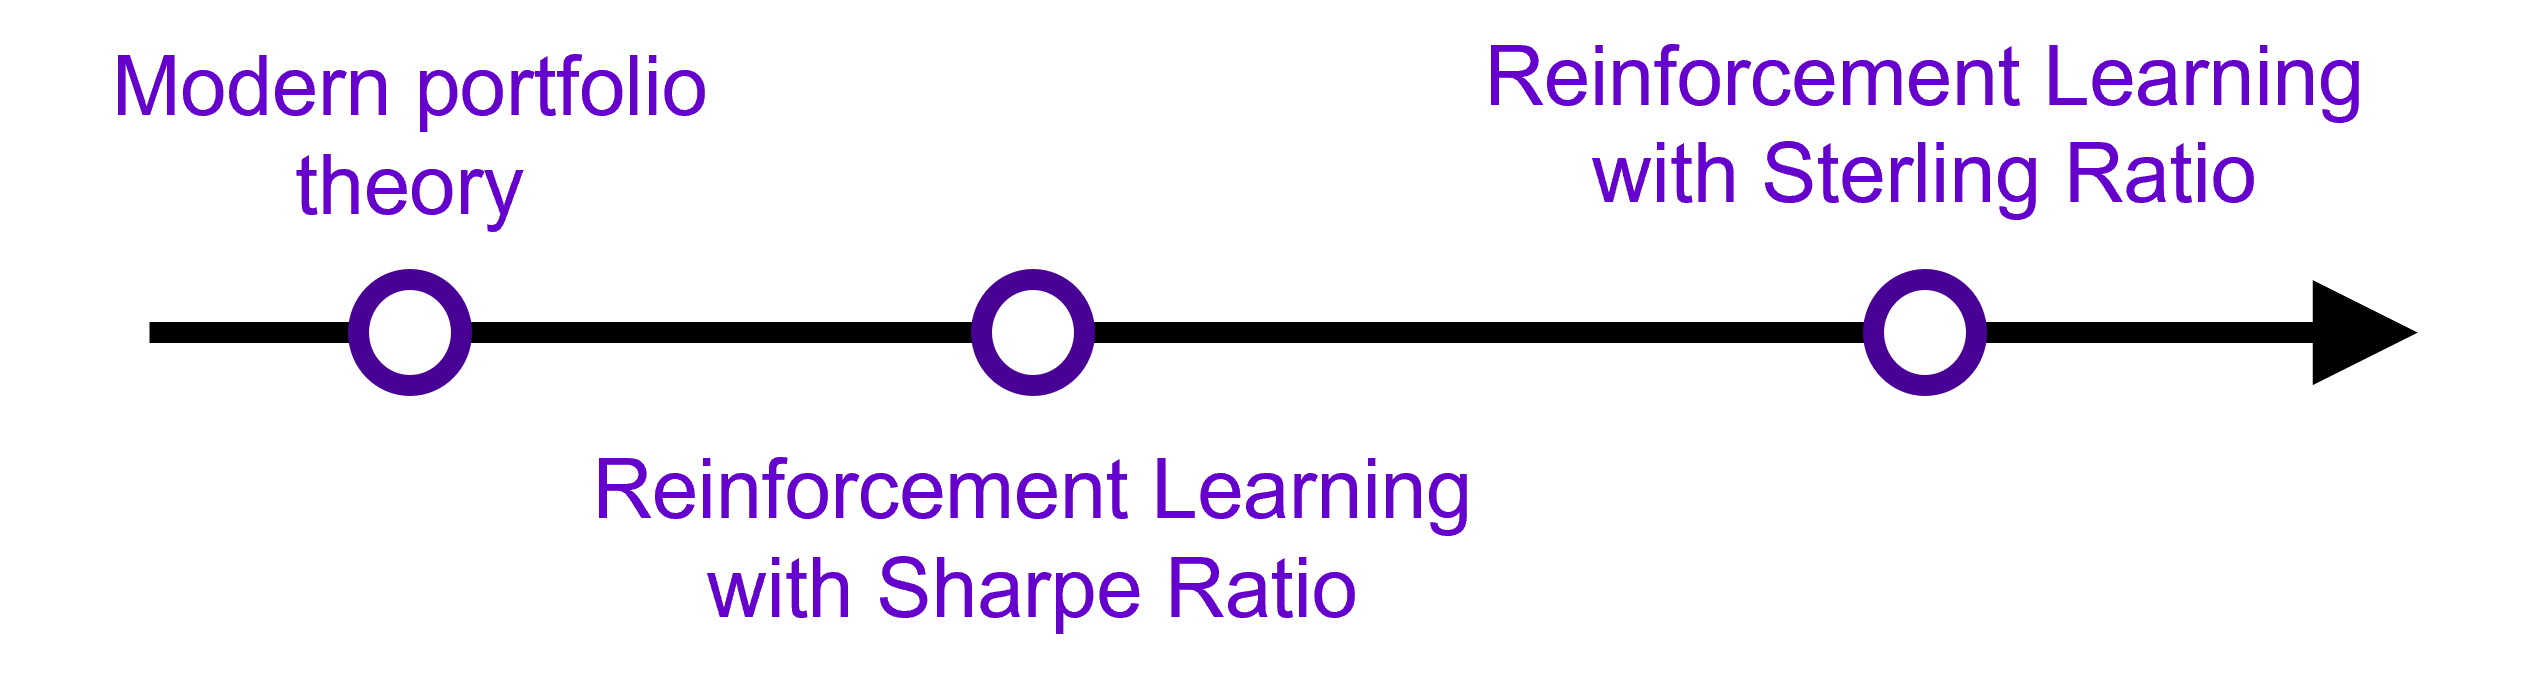
\includegraphics[width=10cm]{images/related.png}
    \end{center}
\end{frame}

\subsection{Modern Portfolio Theory}

\begin{frame}
\frametitle{Modern Portfolio Theory (MPT)}
\begin{columns}
\begin{column}{0.55\textwidth}
\begin{block}{Problem}
    How to construct portfolios with risk preference?
\end{block}
\begin{block}{Solution}
    Choose the portfolio with highest expected return from given risk (variance) by efficient frontier.
\end{block}
\end{column}
\begin{column}{0.45\textwidth}
\begin{center}
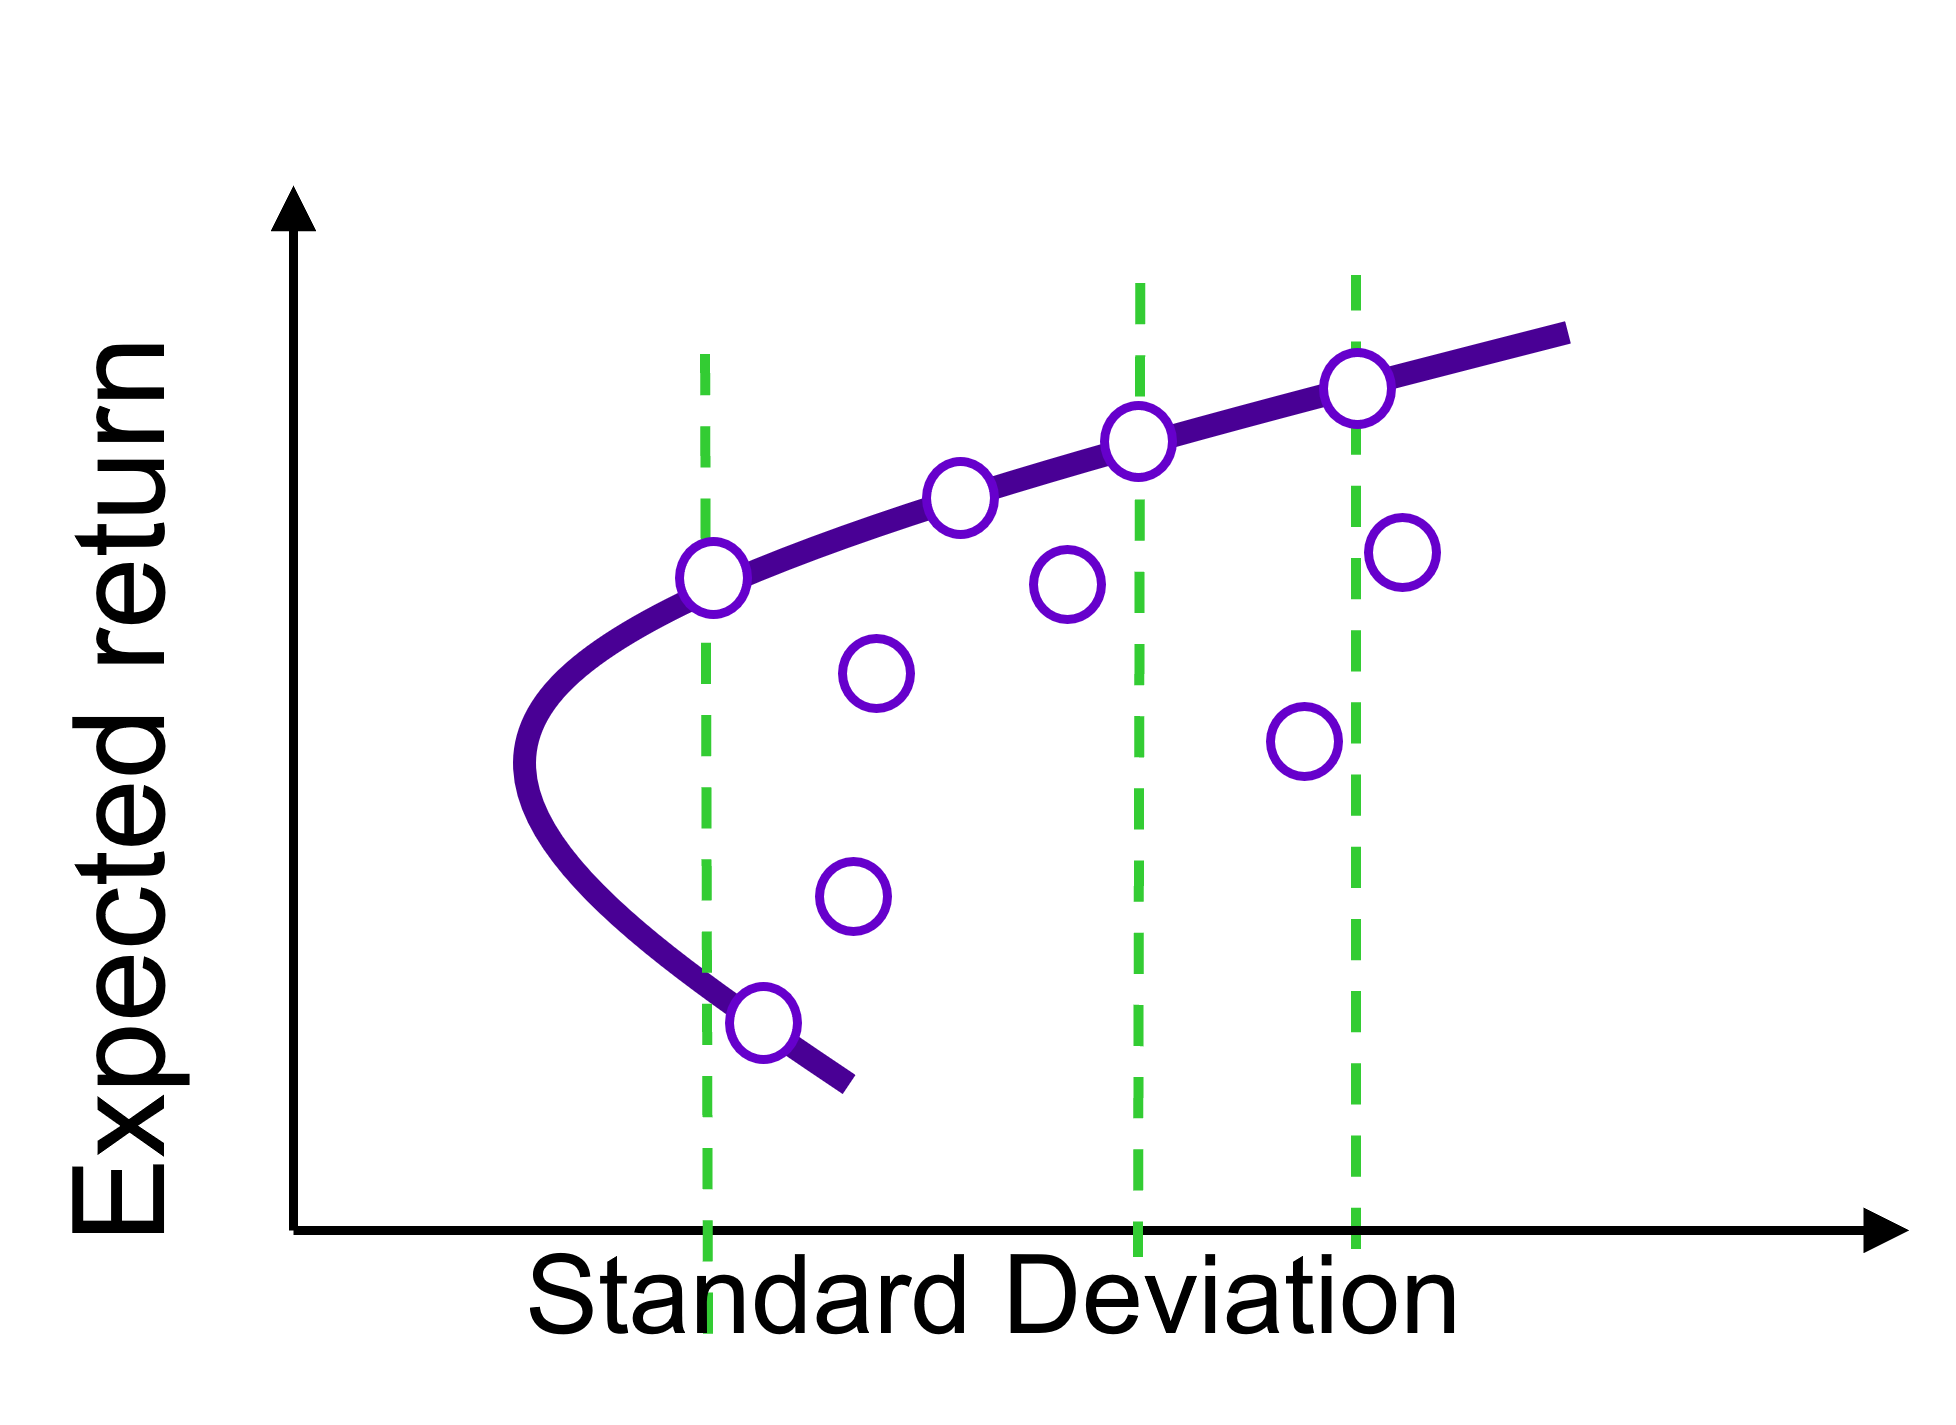
\includegraphics[width=4.8cm]{images/mpt_risk.png}
\end{center}
\end{column}
\end{columns}
\end{frame}

\subsection{Reinforcement Learning with Sharpe Ratio}
\begin{frame}{Reinforcement Learning with Sharpe Ratio}
\begin{block}{Problem}
Loss of information for two staged system, forecasting/trading
\end{block}

\begin{block}{Solution}
Train trading systems and portfolios by optimizing objective
functions, e.g. Sharpe Ratio, directly with Reinforcement Learning.
\end{block}

\begin{block}{Sharpe Ratio}
\[ SharpeRatio = \frac{E(R_a - R_f)}{\sigma_a}\]
\end{block}
\end{frame}



\subsection{Reinforcement Learning with Sterling Ratio}
\begin{frame}{Reinforcement Learning with Sterling Ratio}
\begin{block}{Problem}
Sharpe ratio is criticized for adjustment done based on variance rather than downside risk, \alert {penalty upon large positive returns}.
\end{block}
\begin{block}{Solution}
Use Sterling Ratio as objective function.
\[
Sterling Ratio=\frac{Annualized Average Return}{Maximum Drawdown}
\]
\end{block}

\end{frame}

\begin{frame}{Alternatives to Maximum Drawdown and  Sterling Ratio}
\begin{block}{Problem}
Maximum Drawdown is cumbersome to minimize.
\end{block}

\begin{block}{Solution}
Moody used DD to replace , the square root of the average of the
square of the negative returns, defined as
\[
DD_T = \sqrt{\cfrac{1}{T}\sum_{t=0}^{T}{min\{R_T,0\}^2}}
\]
And replace Sterling Ratio with downside deviation ratio (DDR)
\[
DDR_T = \frac{Average(R_T)}{DD_T}
\]
\end{block}
\end{frame}



\subsection{Comparison}
\begin{frame}{Comparison}
    \begin{block}{MPT}
        \begin{itemize}
            \item \color{ForestGreen}{Adjustable risk preferences}
            \item\alert{Two staged system, loss of information}
        \end{itemize}
    \end{block}
    \begin{block}{RL-based with Sharpe/Sterling Ratio}
        \begin{itemize}    
            \item \alert{No adjustable risk preferences}
            \item \color{ForestGreen}{Optimization directly}    
        \end{itemize}            
    \end{block}

    \begin{block}{Proposed System}
        \begin{itemize}
        \item \color{ForestGreen}{Adjustable risk preferences}
        \item \color{ForestGreen}{Optimization directly}  
        \end{itemize}        
    \end{block}

\end{frame}